% Diagram fungsional berdasarkan diagram pengguna dan program panel.
% Node pertama terpasang; node berikutnya merupakan rancangan pengembangan.
\begin{figure}[tbp]
\centering
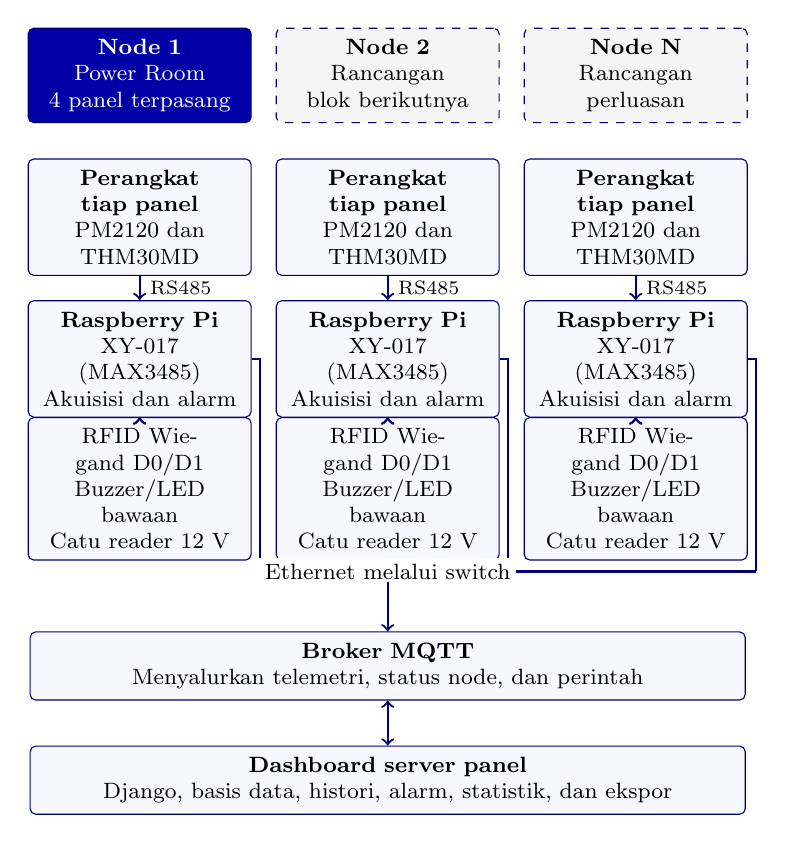
\begin{tikzpicture}[
 font=\rmfamily\fontsize{8}{9.5}\selectfont,
 box/.style={draw=blue!45!black,rounded corners=2pt,align=center,
 fill=blue!3,inner sep=4pt,text width=2.55cm},
 link/.style={->,thick,draw=blue!45!black}]
\node[box,fill=blue!65!black,text=white] at (-3.15,0)
 {\textbf{Node 1}\\Power Room\\4 panel terpasang};
\node[box,dashed,fill=gray!8] at (0,0)
 {\textbf{Node 2}\\Rancangan blok berikutnya};
\node[box,dashed,fill=gray!8] at (3.15,0)
 {\textbf{Node N}\\Rancangan perluasan};
\foreach \x/\name in {-3.15/a,0/b,3.15/c}{
 \node[box] (meter\name) at (\x,-1.8)
  {\textbf{Perangkat tiap panel}\\PM2120 dan THM30MD};
 \node[box] (pi\name) at (\x,-3.6)
  {\textbf{Raspberry Pi}\\XY-017 (MAX3485)\\Akuisisi dan alarm};
 \draw[link] (meter\name) -- node[right,font=\rmfamily\fontsize{7}{8}\selectfont]
  {RS485} (pi\name);
 \node[box] (alarm\name) at (\x,-5.25)
  {RFID Wiegand D0/D1\\Buzzer/LED bawaan\\Catu reader 12 V};
 \draw[<->,thick,blue!45!black] (pi\name) -- (alarm\name);
 \draw[thick,blue!45!black] (pi\name.east) -- (\x+1.53,-3.6) -- (\x+1.53,-6.3);
}
\draw[thick,blue!45!black] (-1.62,-6.3) -- (4.68,-6.3);
\node[fill=white,inner sep=2pt] at (0,-6.3) {Ethernet melalui switch};
\node[box,text width=8.8cm] (broker) at (0,-7.5)
 {\textbf{Broker MQTT}\\Menyalurkan telemetri, status node, dan perintah};
\draw[link] (0,-6.43) -- (broker);
\node[box,text width=8.8cm] (server) at (0,-8.95)
 {\textbf{Dashboard server panel}\\Django, basis data, histori, alarm, statistik, dan ekspor};
\draw[<->,thick,blue!45!black] (broker) -- (server);
\end{tikzpicture}
\caption{Arsitektur monitoring panel dan pengembangan per blok}
\label{fig:panel-arsitektur}
\end{figure}
